\documentclass{jhwhw}
%\everymath{\displaystyle}
\usepackage{color}
%\usepackage{bm}
\usepackage{amsmath}
%\usepackage{setspace}
%\usepackage{verbatim}
\usepackage{graphicx}
%\usepackage[lmargin=2.5cm, rmargin=2.5cm,tmargin=3cm,bmargin=2.5cm]{geometry}
\usepackage{hyperref}
\usepackage{epstopdf}
\usepackage{braket}
\hypersetup{
colorlinks=true,
linkcolor=blue,
urlcolor=blue
}

% This allows you to draw a box around things.
% Wrap whateve you want a box around with:
%\Aboxed{Stuff you want boxed}
\def\@Aboxed#1&#2\ENDDNE{%
  \settowidth\@tempdima{$\displaystyle#1{}$}%
  \addtolength\@tempdima{\fboxsep}%
  \addtolength\@tempdima{\fboxrule}%
  \global\@tempdima=\@tempdima
  \kern\@tempdima
  &
  \kern-\@tempdima
  \fcolorbox{red}{yellow}{$\displaystyle #1#2$}
}

\author{Bret Comnes}
\title{QM619 Homework 1}

\begin{document}
\problem{The Time Energy Uncertainty Principal}
  It is well known that the uncertainty principal in he form of $\Delta E \Delta t \sim h$ has a very different meaning compared to $\Delta p \Delta x \sim h$ since time is \underline{not} an operator in quantum mechanics.  Previously we have introduced one possible interpretation by referring to $\Delta t$ to the ``\emph{amount of time it takes for the expectation value of an observable Q to change by one standard deviation}''.  Here we would like to explore another interpretation of the principle by referring to the first order time-dependent perturbation results.  This approach was first proposed by Landau.  We shall see that the $\Delta t$ according to this will be interpreted as ``\emph{the time it takes to measure a transition energy involving an energy uncertainty of $\Delta E$}''.
  
\part
Let is refer to the case of harmonic time perturbation (similar arguments can be applied to the case of constant perturbation).  For the case of stimulated emission, one can show from Eq. 25.2, Lecture notes, that the first order transition probability can be expressed as:



\begin{equation}
	\label{eq:1otp}
	\left|	c_{f}^{(1)}(t)	\right|^2	
	= 
	4 \left| H_{fi}^{r_0} \right|^2 \left(\frac{t}{2 \hbar}\right)^2 \frac{\sin^2 x}{x^2}
\end{equation}

where 
\begin{equation}
    \label{eq:x}
    x = \left( \frac{E_f-E_i+\hbar\omega}{2\hbar} \right)t
\end{equation}
Give a sketch of $\left|	c_{f}^{(1)}(t)	\right|^2$ as a function of $x$.
\solution

\begin{figure}[htbp]
	\centering
		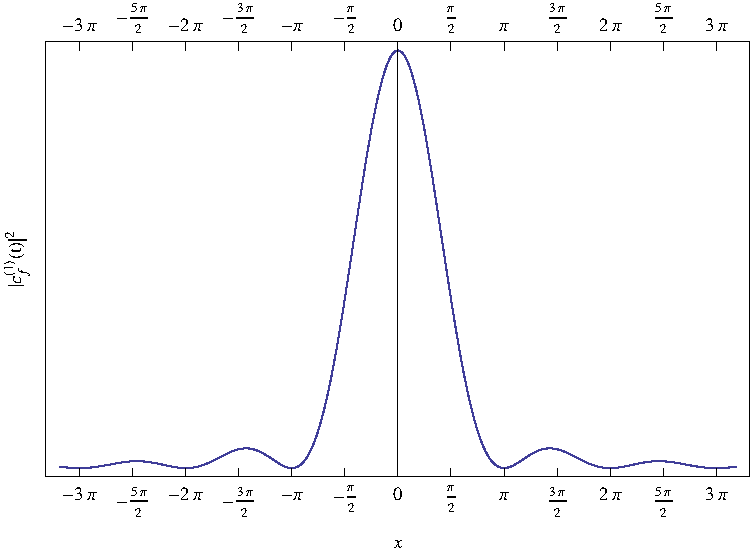
\includegraphics[height=3in]{figures/sinc.pdf}
	\caption{Sketch of $\left|	c_{f}^{(1)}(t)	\right|^2$ as a function of $x$}
	\label{fig:figures_sinc}
\end{figure}
\pagebreak[4]


\part
Let us consider a system (e.g. an atom) and we are measuring the energy states $E_m$ and $E_n(<E_m)$.  We do this by by using a macroscopic apparatus to induce the atom to make a transition from $E_m$ to $E_n$ and measure the emitted photon energy $(\hbar\omega)$ by means of the same apparatus.  The value of the measured photon energy can in principle be assumed knowable exactly.  Try to use the result in a. to introduce a relevant time duration $\Delta t$ and hence formulate the time-energy uncertainty principal in this context.

\solution
We see from the plot in part (a) that there is a central peak around $x = 0$ and it rapidly drops off when $ x < \pi$ indicating that there is a negligible transition probability beyond that point.  Introducing $\Delta t$, the time it takes for the transition form energy state $E_m$ to $E_n$ to occur, to Equation~\eqref{eq:x} we arrive at the condition for stimulated emission.  
\begin{equation}
    x = \left( \frac{E_f-E_i+\hbar\omega}{2\hbar} \right)\Delta t < \pi
\end{equation}

Remembering that $\Delta E = E_f - E_i$ is the energy difference between the two energy levels, and that $\Delta E = \hbar \omega$ is the energy emitted by the photon during stimulation, we can simplify this further:
\begin{align}
    \left( \frac{2 \Delta E}{2\hbar} \right)\Delta t &< \pi \\
    \Delta t \Delta E &< \hbar \pi \\
    \label{eq:tup}
    \Delta t \Delta E &\approx h
\end{align}

\part
Can you generalize the above to introduce the concepts of ``line width'' and ``lifetime'' for an excited state of an atomic system and establish a relationship between them?

\solution
We can define a transition probability per unit time, $W$ by summing the individual transmission probabilities \eqref{eq:1otp} and dividing it by time.
\begin{align}
    W = \frac{1}{t}\sum \limits_f \left|	c_{f}^{(1)}(t)	\right|^2
\end{align}
From here, we can define a ``lifetime'' as
\begin{equation}
    \tau = \frac{1}{W}
\end{equation}
which is referred to as the ``Golden Rule''.

From the time uncertainty principal \eqref{eq:tup}, we can define a ``line width'' of the excited state m as
\begin{equation}
    \Gamma_m \equiv \Delta E_m = \frac{h}{\tau}
\end{equation}
by substituting $\Delta E \rightarrow \Delta E_m$ and $t \rightarrow \tau$. 

\problem{The Thomas-Reiche-Kuhn (TRK) sum rule}
\textbf{A. Approach 1:}
The dipole oscillator strength $f_{mn}$ is a very useful quantity in calculating intensities of spectral lines in atomic physics.  In terms of the dipole transition matrix elements, the oscillator strength is defined as:

\begin{equation}
	\label{eq:fmn}
	f_{mn}=f_{mn}^x + f_{mn}^y + f_{mn}^z = \frac{2 m \omega_{mn}}{\hbar}\left[|x_{mn}|^2 + |y_{mn}|^2 + |z_{mn}|^2 \right]
\end{equation}

where 
\begin{align}
	\hbar \omega_{mn} &= E_m - E_n \\
	\label{eq:xmn0}
	x_{mn} &= \int u_m^* x u_n d\tau \text{...etc.}
\end{align}

\part Show that $f_{mn}^*$ can be written in a slightly different form as:
\begin{equation}
	\label{eq:fmnstar}
	f_{mn}^* = \frac{m}{\hbar}(\omega_{mn} x_{mn} x_{nm} - \omega_{nm} x_{nm} x_{mn})
\end{equation}
\solution
Lets first by establishing some useful relationships.  Looking at $x_{mn}$ and $x_{nm}$:
\begin{align}
	x_{mn}^* &= \int u_n^* x u_m d\tau \\
	x_{nm} &= \int u_n^* x u_m d\tau \\
	x_{nm} &= x_{mn}^*
\end{align}
we also see the relationship between $\omega_{mn}$ and $\omega_{nm}$:
\begin{align}
	\hbar \omega_{mn} &= E_m - E_n \\
	\hbar \omega_{nm} &= E_n - E_m \\
	-\hbar \omega_{mn} &= E_n - E_m \\
	-\hbar \omega_{mn} &= \hbar \omega_{nm} \\
	\label{eq:xmn}
	-\omega_{mn} &= \omega_{nm}	
\end{align}
such that
\begin{align}
	2 \hbar \omega_{mn}	&= 2(E_m - E_n) \\
					&= E_m - E_n - E_n + E_m \\
					&= \hbar \omega_{mn} - \hbar \omega_{nm} \\ 
					\label{eq:omega2}
	2 \omega_{mn}	&= \omega_{mn} - \omega_{nm}
\end{align}
Now we can start plugging in Equation~\eqref{eq:xmn} and Equation~\eqref{eq:omega2} to $f_{mn}^x$.
\begin{align}
f_{mn}^x 	&= \frac{2 m \omega_{mn}}{\hbar}\left|x_{mn}\right|^2 \\
			&= \frac{m}{\hbar} (\omega_{mn} - \omega_{nm}) \left|x_{mn}\right|^2 \\
			&= \frac{m}{\hbar} (\omega_{mn} - \omega_{nm}) x_{mn}^* x_{mn} \\
			&= \frac{m}{\hbar} (\omega_{mn} - \omega_{nm}) x_{mn} x_{nm} \\
			\label{eq:fmnxw}
\Aboxed{f_{mn}^x	&= \frac{m}{\hbar} (\omega_{mn} x_{mn} x_{nm}  - \omega_{nm} x_{mn} x_{nm} )} 
\end{align}

\pagebreak[4]

\part 
From the procedures shown in the Lecture Notes [Eq. ($25.16$)-($25.18$)], show that 
\begin{equation}
	\label{eq:pxmn}
	(p_x)_{mn} =i m \omega_{mn}x_{mn}
\end{equation}
where $(p_x)_{mn}$ is the transition matrix element for the x-component of the momentum and m is the mass of the electron.
\solution
From the notes (25.17), we know that
\begin{equation}
    \label{eq:xhcom}
	[x_i,H_0] = \frac{1}{2m}[x_i,p_i^2] = \frac{1}{2m} [x_i,p_i]p_i + \frac{1}{2m}p_i[x_i,p_i] = \frac{i \hbar}{m}p_i
\end{equation}
where
\begin{equation}
	[x_i,p_i] = i \hbar
\end{equation}
from the quantum condition.  In order to find $(p_x)_{mn}$ we need to operate on $\braket{m|n}$ with $[x,H_0]$ and solve for $p_x$ to find the $mn$'th element of $p_x$.
\begin{align}
	\bra{m}[x,H_0]\ket{n} &= \frac{i \hbar}{m}(p_x)_{mn} & & \\
	\bra{m} x H_0 - H_0 x\ket{n} &=  & &  \\
	(E_n - E_m )\bra{m} x \ket{n} &=  & &\text{where }(E_n - E_m ) = -\hbar \omega_{mn}  \\
	- \hbar \omega_{mn} x_{mn} &=  & &\text{and } \bra{m} x \ket{n} = x_{mn}  \\
	- \frac{m}{i \hbar} \hbar \omega_{mn} x_{mn} &= (p_x)_{mn}  & &  \\
	\Aboxed{(p_x)_{mn} &= i m \omega_{mn} x_{mn}}  & & 
\end{align}

\pagebreak[4]

\part
Hence, using (a) and (b), show that $f_{mn}^*$ can be written as:

\begin{equation}
	\label{eq:fmnxp}
	f_{mn}^x = \frac{i}{\hbar}\left(p_{nm}x_{mn}-x_{nm}p_{mn}\right)
\end{equation}

\solution
Comparing Equation~\eqref{eq:fmnxw} and Equation~\eqref{eq:pxmn}, we see that it will be useful to write
\begin{align}
    \frac{(p_x)_{mn}}{i m} &= \omega_{mn}x_{nm} & \frac{(p_x)_{nm}}{i m} &= \omega_{nm}x_{mn}
\end{align}
which can be substituted into Equation~\eqref{eq:fmnxw} directly.
\begin{align}
    f_{mn}^x	&= \frac{m}{\hbar} \left(\frac{(p_x)_{mn}}{i m} x_{nm}  - \frac{(p_x)_{nm}}{i m} x_{m n} \right) \\
    &= \frac{1}{i \hbar} \left((p_x)_{mn} x_{nm}  - (p_x)_{nm} x_{mn} \right) \\
    \Aboxed{f_{mn}^x &= \frac{i}{\hbar}  ((p_x)_{nm} x_{mn} - (p_x)_{mn} x_{nm} )}\\
\end{align}

\pagebreak[4]

\part
Using the closure property of the wave functions in the following form: 

\begin{equation}
	\label{eq:dr}
\sum\limits_{m} u_m^* (\vec{r}) u_{m}(\vec{r'})= \partial(\vec{r} - \vec{r'})
\end{equation}
(can you prove this?), derive the following TRK sum rule:
\begin{align}
	\sum\limits_m f_{mn}^x &= 1 \\ \sum\limits_m f_{mn} &= 3
\end{align}

\solution
No Dirac notation allowed!  Or at least any of the fancy shortcuts it prohibits.  This is a messy operation so hang on tight.  Since $ \sum\limits_m f_{mn}$ is simply the sum of $\sum\limits_m f_{mn}^x$, $ \sum\limits_m f_{mn}^y$ and $\sum\limits_m f_{mn}^z$ \footnote{See Equation~\eqref{eq:fmn}}, all we need to do is find one and we have the others.  Lets find $\sum\limits_m f_{mn}^x$.
\begin{align}
    \sum\limits_m f_{mn}^x &= \sum\limits_m\frac{i}{\hbar}  ((p_x)_{nm} x_{mn} - (p_x)_{mn} x_{nm} ) \\
    \label{eq:bignasty}
    &= \frac{i}{\hbar}  (\sum\limits_m(p_x)_{nm} x_{mn} - \sum\limits_m(p_x)_{mn} x_{nm} )
\end{align}
We know from Equation~\eqref{eq:xmn0} that
\begin{align}
    x_{mn} &= \int u_m^* x u_n d\tau & (p_x)_{mn} &= \int u_m^* p_x u_n d\tau \\
    x_{nm} &= \int u_n^* x u_m d\tau & (p_x)_{nm} &= \int u_n^* p_x u_m d\tau
\end{align}
so that at this point Equation~\eqref{eq:bignasty} is a matter of tedious algebra, notation and calculus trickery.  It is at this point that I begin clamoring for Dirac notation, but its not allowed.  
\begin{align}
    \sum\limits_m f_{mn}^x &= \frac{i}{\hbar}  (\sum\limits_m(p_x)_{nm} x_{mn} - \sum\limits_m(p_x)_{mn} x_{nm} ) \\
    &= \frac{i}{\hbar}  
    \left(
    \sum\limits_m \int u_n^*(\vec{r'}) p_x u_m(\vec{r'}) d\tau' \int u_m^*(\vec{r}) x u_n(\vec{r}) d\tau - 
    \sum\limits_m \int u_m^*(\vec{r'}) p_x u_n(\vec{r'}) d\tau' \int u_n^*(\vec{r}) x u_m(\vec{r}) d\tau
    \right)
    \\
    &= \frac{i}{\hbar}  
      \left(
      \int \int \sum\limits_m u_n^*(\vec{r'}) p_x u_m(\vec{r'}) u_m^*(\vec{r}) x u_n(\vec{r}) d\tau' d\tau - 
      \int \int \sum\limits_m u_m^*(\vec{r'}) p_x u_n(\vec{r'}) u_n^*(\vec{r}) x u_m(\vec{r}) d\tau' d\tau
      \right)
\end{align}
Using the closure property see in Equation~\eqref{eq:dr} and the fact $\delta{x} = \delta{-x}$ we see that our discrete summation reduced to Dirac delta functions.
\begin{align}
    \sum\limits_m f_{mn}^x &= \frac{i}{\hbar}  
      \left(
      \int \int u_n^*(\vec{r'}) p_x \delta(\vec{r}-\vec{r'}) x u_n(\vec{r}) d\tau' d\tau - 
      \int \int u_n^*(\vec{r}) x \delta(\vec{r}-\vec{r'}) p_x u_n(\vec{r'}) d\tau' d\tau
      \right)
\end{align}
Performing one of the integrals we see that $\vec{r'} = \vec{r}$ due to the delta functions, otherwise the matrix elements are of 0 value.
\begin{align}
    \sum\limits_m f_{mn}^x &= \frac{i}{\hbar}  
      \left(
      \int u_n^*(\vec{r}) p_x x u_n(\vec{r}) d\tau - 
      \int u_n^*(\vec{r}) x p_x u_n(\vec{r}) d\tau
      \right)
\end{align}
At this point the math is just screaming commutator rules, but we mush push on.  Remembering that $p_x = (- i \hbar) \frac{d}{dx}$
\begin{align}
    \sum\limits_m f_{mn}^x &= \frac{i}{\hbar}  
      \left(
      \int u_n^*(\vec{r}) (- i \hbar) \frac{d}{dx} x u_n(\vec{r}) d\tau - 
      \int u_n^*(\vec{r}) x (- i \hbar) \frac{d}{dx} u_n(\vec{r}) d\tau
      \right) \\
      &= \left(
        \int u_n^*(\vec{r})  \frac{d}{dx} x u_n(\vec{r}) d\tau - 
        \int u_n^*(\vec{r}) x  \frac{d}{dx} u_n(\vec{r}) d\tau
        \right) \\
    &= \left(
    \int u_n^*(\vec{r})  \frac{dx}{dx} u_n(\vec{r})d\tau + \int u_n^*(\vec{r}) x \frac{d u_n(\vec{r})}{dx} d\tau - 
    \int u_n^*(\vec{r}) x  \frac{du_n(\vec{r})}{dx} d\tau
    \right) \\
    &= \left(
    \int u_n^*(\vec{r})  \frac{dx}{dx} u_n(\vec{r})d\tau
    \right) \\
    \Aboxed{\sum\limits_m f_{mn}^x &= 1}
\end{align}
using the closure property.  Finally,
\begin{align}
    \sum\limits_m f_{mn} &= \sum\limits_m f_{mn}^x + \sum\limits_m f_{mn}^y + \sum\limits_m f_{mn}^z \\
    \Aboxed{\sum\limits_m f_{mn} &= 1 + 1 + 1 = 3}
\end{align}
I get it.  Dirac notation is really nice sometimes, as a simple $\bra{u_m}[x,p_x]\ket{u_n} = -i \hbar$ would really be nice about now.

\pagebreak[4]

\textbf{B. Approach 2:}
Let us re-derive the above sum rule using Dirac notation.  We shall see the beautiful result for closure obtained in this notation, i.e.: $\sum\limits_k \ket{k}\bra{k} = 1$ will lead to a much simpler proof of the above result.  It is sufficient for us to just derive the result of the x-dipole transition matrix element here.  Consider a non-relativistic atom with Hamiltonian:

\begin{align}
	\label{eq:Ham}
	H &= \frac{\vec{p}^2}{2m}+V(r) & \vec{r} &= (x,y,z)
\end{align}
\part
Use the quantum condition to derive the following result for the ``double commutator'':

\begin{equation}
	\label{eq:double}
	\left[x, \left[x,H \right] \right] = - \frac{\hbar^2}{m}
\end{equation}
\solution
Looking back to the notes (25.17) or Equation~\eqref{eq:xhcom} we know
\begin{align}
    \label{eq:xhpcomm}
    [x_i,H_0] = \frac{i \hbar}{m}p_i
\end{align}
Simply plugging this into Equation~\eqref{eq:double} and using the quantum condition we arrive at our goal:
\begin{align}
    \left[x,\frac{i \hbar}{m}p_i \right] &=  \frac{i \hbar}{m} \left[x,p_i \right] = \frac{i \hbar}{m} i \hbar \\
    \Aboxed{\left[x, \left[x,H \right] \right] &= - \frac{\hbar^2}{m}}
\end{align}

\part
Hence derive the TRK sum rule in the form:

\begin{equation}
	\label{eq:trk}
	\sum\limits_k \left( E_k - E_n \right) \left| x_{k n} \right|^2 = \frac{\hbar^2}{2m} \text{, where } x_{k n} = \bra{k}x\ket{n} \text{ and } H\ket{n} = E_n \ket{n}
\end{equation}

\solution
Following the hint's give in Gasiorowicz we can write the quantum condition as:
\begin{align}
    \bra{n}[p,x]\ket{n} &= - i \hbar \\
    \bra{n}px - xp\ket{n} &= - i \hbar \\
    \bra{n} p x \ket{n} - \bra{n} x p\ket{n} &= - i \hbar 
\end{align}
using closure
\begin{align}
    \label{eq:gashint}
    \sum \limits_k \bra{n} p \ket{k} \bra{k} x \ket{n} - \sum \limits_k \bra{n} x \ket{k} \bra{k} p \ket{n} &= - i \hbar
\end{align}

Solving \eqref{eq:xhpcomm} for $p$, we can sub into \eqref{eq:gashint}

\begin{align}
    [x_i,H_0] &= \frac{i \hbar}{m}p_i \\
    \frac{m}{i \hbar} [x_i,H_0] &= p_i
\end{align}
so that
\begin{align}
    \frac{m}{i \hbar} \left( \sum \limits_k \bra{n} [x_i,H_0]\ket{k}\bra{k}x\ket{n} - \sum \limits_k\bra{n}x\ket{k}\bra{k} [x_i,H_0]\ket{n} \right) &= - i \hbar \\
    \frac{m}{i \hbar} \left( \sum \limits_k (E_k - E_n) \bra{n} x \ket{k}\bra{k}x\ket{n} +  \sum \limits_k (E_k - E_n)\bra{n}x\ket{k}\bra{k} x \ket{n} \right) &= - i \hbar \\
    \frac{m}{i \hbar} \left( \sum \limits_k (E_k - E_n) \bra{k} x \ket{n}^*\bra{k}x\ket{n} +  \sum \limits_k (E_k - E_n)\bra{k}x\ket{n}^*\bra{k} x \ket{n} \right) &= - i \hbar \\
    \frac{m}{i \hbar} \left( \sum \limits_k (E_ - E_n) \left|\bra{k}x\ket{n}\right|^2 +  \sum \limits_k (E_k - E_n)\left|\bra{k}x\ket{n}\right|^2 \right) &= - i \hbar \\
    \frac{2 m}{i \hbar}  \sum \limits_k (E_k - E_n) \left|\bra{k}x\ket{n}\right|^2  &= - i \hbar \\
    \sum \limits_k (E_k - E_n) \left|\bra{k}x\ket{n}\right|^2  &=  \frac{\hbar^2}{2m} \\
    \Aboxed{\sum \limits_k (E_k - E_n) \left|x_{kn}\right|^2  &=  \frac{\hbar^2}{2m}}
\end{align}

\problem{The adiabatic Theorem}
This theorem states that if the Hamiltonian of a system is changed very slowly from $H_0$ to $H$, then the system in a given eigenstate of $H_0$ will simply go over the corresponding eigenstate of $H$, without making any transitions.  To illustrate this, let us a system being in the ground state $u_0$ of $H_0$ defined by : $H_0 u_0 = E_0^0 u_0$.  Now let $H_0$ go over very slowly to $H = H_0 + V$, $V$ being small, the theorem requires that the state of the system must go over from $u_0$ to the ground state $w_0$ of $H$, defined by $H w_0 = E_0 w_0$.  Let is prove this as follows:

\part

Consider a time-dependent perturbation to $H_0 : H'(t) = f(t)V$ where $f(t)$ is a slowly varying function from 0 to 1 as shown.  Using integration by parts, establish the following results for the integral:

\begin{equation}
	\label{eq:byparts}
	\int_0^t f(t') e^{i \omega_{mn}t'} dt' = \int_0^t f(t')\frac{1}{i \omega_{mn}}\frac{d}{dt'} e^{i \omega_{mn}t'}dt' \approx \frac{1}{i \omega_{mn}} f(t) e^{i \omega_{mn} t}
\end{equation}

\solution
We will use simple integration by parts:
\begin{equation}
    \int f(x)g'(x)dx = f(x)g(x) - \int g(x)f'(x)dx
\end{equation}
Selecting f and g to be:
\begin{align}
    f &= f(t') & g' &= \frac{1}{i \omega_{mn}}\frac{d}{dt}e^{i \omega_{mn} t'} = e^{i \omega_{mn} t'} \\
    f' &= \frac{df(t')}{dt'} & g &= \frac{1}{i \omega_{mn}}e^{i \omega_{mn} t'}
\end{align}
we can perform the integral now
\begin{align}
    \int_0^t f(t')\frac{1}{i \omega_{mn}}\frac{d}{dt'} e^{i \omega_{mn}t'}dt' &= 
    f(t')\frac{1}{i \omega_{mn}}e^{i \omega_{mn} t'}\bigg|_0^t - \int_0^t \frac{1}{i \omega_{mn}}e^{i \omega_{mn} t'} \frac{df(t')}{dt'} dt'
\end{align}
We can drop the second term because our system is going through an adiabatic transition, meaning that that the time derivative of $f$ is going to be nearly 0, so we are left with:
\begin{align}
   \Aboxed{\int_0^t f(t')\frac{1}{i \omega_{mn}}\frac{d}{dt'} e^{i \omega_{mn}t'}dt' &\approx \frac{1}{i \omega_{mn}} f(t) e^{i \omega_{mn} t}}
   \label{eq:intaprox}
\end{align}
\pagebreak[4]

\part
Using first order time-dependent perturbation theory, show that the time-dependent wave function $ \Psi(t) $ can be expressed as :

\begin{align}
	\label{eq:PSI}
	\Psi(t) &= \sum\limits_{n}c_n (t) e^{-i \omega_m t} u_n \\
	\text{where } \omega_n &= E_n^0 / \hbar
\end{align}
and the coefficients $c_n(t)$ are given by
\begin{equation}
	\label{eq:c0}
	c_0 = 1 + \frac{1}{i \hbar} V_{0 0} \int_0^t f(t') dt'
\end{equation}
and for $n \neq 0$,
\begin{align}
	\label{eq:cn}
	c_n &= \frac{1}{i \hbar} V_{n0} \int_0^t f(t') e^{i \omega_{n0} t'} dt' \\
	\text{with } V_{n0} &= \int u_n^* V u_0 d\tau \\
	\label{eq:wn0}
	\text{and }\omega_{n0} &= \frac{ E_n^0 - E_0^0}{\hbar}
\end{align}
\solution
Lets find $\Psi(x)$ for a system made up of a single eigenfunction then generalize to the full set of eigenfunctions, following Griffiths 2nd edition page 371.  If the system is in the $n$'th eigenstate we have
\begin{align}
    H \psi_n &= E_n \psi_n & \braket{\psi_n|\psi_m} &= \delta_{nm}
\end{align}
At time $t = 0$ we perturb the system so that the total Hamiltonian is
\begin{equation}
    H = H_0 + H'(t)
\end{equation}
which when we generalize our perturbed two state system
\begin{equation}
    \Psi(t) = c_a(t)\psi_a e^{-i E_a t / \hbar} + c_b(t)\psi_b e^{-i E_b t \hbar}
\end{equation}
reads
\begin{align}
    \Aboxed{\Psi(t) &= \sum c_n(t) \psi_n e^{-i E_n t \ \hbar}}
\end{align}
where
\begin{align}
    \Aboxed{c_n(t) &\approx 1 - \frac{i}{\hbar} \int_0^t H'_{n n}(t')dt'} \\
    \Aboxed{c_{m \neq n}(t) &\approx \frac{-i}{\hbar}\int^t_0 H'_{m n}(t')e^{i(E_m - E_n)t'/\hbar}dt'}
\end{align}
\begin{equation}
    \Psi_n = \psi_n e^{-i E_n t / \hbar} 
\end{equation}

\pagebreak[4]
\part
Using the results in a, show that for large t:

\begin{equation}
	\label{eq:larget}
	\Psi(t) \approx \left[\left( 1 - i \frac{V_{00}A}{\hbar}\right)u_0 - \sum\limits_{n \neq 0} \frac{V_{n0}}{E_n^0-E_0^0}u_n \right]e^{-i \omega_0 t}
\end{equation}
where 
\begin{equation}
     \label{eq:A}
    A = \int^t_0 f(t')dt'
\end{equation}


\solution
Using the results from (A) Equation~\eqref{eq:PSI}
\begin{align}
    \Psi(t) &= \sum\limits_{n}c_n (t) e^{-i \omega_n t} u_n
\end{align}
At this point we just start filling this out, separating out $n = 0$ and $ n \neq 0$.  Using Equations~\eqref{eq:c0} - \eqref{eq:wn0}
\begin{align}
    \Psi(t) &\approx \left(1 - \frac{i V_{00}}{\hbar} \int_0^t  f(t') dt'\right)e^{-i \omega_0 t}u_0 + \sum\limits_{n \neq o}c_n (t) e^{-i \omega_n t} u_n & \text{Using Eq. \eqref{eq:A}} \\
    \Psi(t) &\approx \left(1 - \frac{i V_{00}}{\hbar} A\right)e^{-i \omega_0 t}u_0 + \sum\limits_{n \neq o}c_n (t) e^{-i \omega_n t} u_n & & \\
    \Psi(t) &\approx \left(1 - \frac{i V_{00}}{\hbar} A\right)e^{-i \omega_0 t}u_0 + \sum\limits_{n \neq o}\left( \frac{-V_{n0}}{\hbar \omega_{n0}} f(t) e^{i \omega_{n0}t} e^{-i \omega_n t}u_n\right) & \text{using Eq.} \eqref{eq:intaprox}& \\
    \Psi(t) &\approx \left[ \left(1 - \frac{i V_{00}}{\hbar} A u_0\right) + \sum\limits_{n \neq o}\left( \frac{-V_{n0}}{\hbar \omega_{n0}} f(t) u_n\right) \right]e^{-i \omega_0 t} & e^{i t(\omega_{n0} - \omega_n)} = e^{-i\omega_0 t}& \\
    \Psi(t) &\approx \left[ \left(1 - \frac{i V_{00}}{\hbar} A u_0\right) + \sum\limits_{n \neq o}\left( \frac{-V_{n0}}{E_n^0 - E_0^0} f(t) u_n\right) \right]e^{-i \omega_0 t} & \text{using Eq. } \eqref{eq:wn0}& \\
     \Aboxed{\Psi(t) &\approx \left[ \left(1 - \frac{i V_{00}}{\hbar} A u_0\right) + \sum\limits_{n \neq o}\left( \frac{-V_{n0}}{E_n^0 - E_0^0} u_n\right) \right]e^{-i \omega_0 t}} & f(t \rightarrow \infty) = 1&
\end{align}

\pagebreak[4]
\part
From the time-independent perturbation theory we have: 
\begin{equation}
	\label{eq:tipt}
	w_0 = u_0 + \sum\limits_{k \neq 0} \frac{V_{k0}}{E_0^0 - E_k^0}u_k
\end{equation}

Use the results in c. to show that:

\begin{equation}
	\label{eq:braket}
	\left|\braket{ \Psi(t) | w_0 }\right|^2 \equiv \left| \int \Psi^*(t)w_0 d\tau \right|^2 \rightarrow 1 \text{ to the first order in } V
\end{equation}
\solution
First lets find $\braket{\Psi(t)w_0}$:
\begin{align}
	\int \Psi^*(t)w_0 d\tau &= \int \left[ \left( \left(1 + \frac{i V_{00}}{\hbar} A u_0^*\right) + \sum\limits_{n \neq o}\left( \frac{-V_{n0}}{E_n^0 - E_0^0} u_n^*\right)\right)  \left(u_0 + \sum\limits_{k \neq 0} \frac{V_{k0}}{E_0^0 - E_k^0}u_k\right)\right]e^{+i \omega_0 t} d\tau
\end{align}
Remember that anytime you get higher than the first order terms of $V$ you drop that part of the result.  Also, remember Equation \eqref{eq:dr} of orthogonality.  With these two things in mind, we should see this reduce down to the desired result.
\begin{align}
	\int \Psi^*(t)w_0 d\tau =  \int \bigg[ \left( u_0 + \frac{i V_{00}}{\hbar} A u_0^*u_0\right) + \sum\limits_{n \neq o}\left( \frac{-V_{n0}}{E_n^0 - E_0^0} u_n^*u_0\right) \\
	 + \left(u_0 + \frac{i V_{00}}{\hbar} A u_0^*\right)  \sum\limits_{k \neq 0} \left( \frac{V_{k0}}{E_0^0 - E_k^0}u_k\right) + \sum\limits_{n \neq o}\left( \frac{-V_{n0}}{E_n^0 - E_0^0} u_n^*\right)\sum\limits_{k \neq 0} \left( \frac{V_{k0}}{E_0^0 - E_k^0}u_k\right) \bigg]e^{+i \omega_0 t} d\tau \\
\end{align}



\pagebreak[4]

\problem{Energy Time Commutator}
In the Hilbert space formalism of quantum mechanics, the equation of motion of a system given by the quantum condition expressed in terms of the commutators of paris of conjugate variable.  When one projects these back to a certain specific representation, one obtains back the corresponding familiar ``wave equations'' in conventional wave mechanics.  For example, $[\hat{x},\hat{p}] = i \hbar$ leads back to the ``momentum wave equation'' in the coordinate representation:

\begin{equation}
	\label{eq:mwe}
	\left(\frac{\hbar}{i} \frac{\partial}{\partial x} - p\right)\Psi_p (x) = 0
\end{equation}

Hence, \emph{if one can also have an ``energy-time commutator'':} $[\hat{H},\hat{t} = i \hbar]$, with the energy and time both represented by self-adjoint operators, then one would expect the TDSE:
\begin{equation}
	\label{eq:tec}
	\left(\hbar i \frac{\partial}{\partial t} - H\right)\Psi_E (x) = 0
\end{equation}
should also be obtained in the x--representation.  However, one can show (Pauli, 1933) that such a self-adjoint operator for $\hat{t}$ can never exist (see below).  Hence one should regard the operator representation of $\hat{H}: \hat{H}= i \hbar \frac{\partial}{\partial t}$ as a separate postulate in the formulation of Q.M.\footnote{ In classical mechanincs, it is known that H is the generator of time evolution (Goldstein, 2nd ed., p.407-408).  Therefore, if one \emph{postulates} that it \emph{plays the same role in Q.M., then one can also establish TDSE in this way (Ref.: excerpt from ``Quantum Mechanics by Peebles.'')}}
 and is valid in any representation.  To demonstrate Pauli's proof:
 
\part
Let $E_a$ and $\Psi_a$ be certain eigenvalue and eigenfunction of $\hat{H} : \hat{H} \Psi_a = E_a \Psi_a$.  Show that if such a $\hat{t}$ operator exists such that $[\hat{H},\hat{t}] = i \hbar$, then the following eigenvalue equation will be valid:

\begin{equation}
	\label{eq:hbareve}
	\hat{H} \left(e^{i \varepsilon \hat{t} / \hbar} \Psi_a \right) = (E_a - \varepsilon)\left(e^{i \varepsilon \hat{t} / \hbar} \Psi_a \right)
\end{equation} 
where $\varepsilon$ is an arbitrary real constant.\footnote{
\textbf{Hint}: Try to establish the result for the following commutator:
\begin{equation}
	\label{eq:4hint}
	\left[\hat{H}, e^{i \varepsilon \hat{t} / \hbar} \right] = - \left(\frac{i \varepsilon}{\hbar} \right) (-i \hbar) e^{i \varepsilon \hat{t} / \hbar} = -\varepsilon e^{i \varepsilon \hat{t} / \hbar}
\end{equation}}
\solution
Following the advice of the hint, the first thing we do is to establish the commutator from Equation~\eqref{eq:4hint}.
\begin{align}
    \left[
    \hat{H}, e^{i \varepsilon \hat{t} / \hbar} 
    \right] 
    \psi &=  \hat{H} e^{i \varepsilon \hat{t} / \hbar} \psi - e^{i \varepsilon \hat{t} / \hbar} \hat{H} \psi & & \\
    &= i \hbar \frac{\partial}{\partial t}e^{i \varepsilon \hat{t} / \hbar} \psi - e^{i \varepsilon \hat{t} / \hbar} i \hbar \frac{\partial}{\partial t} \psi & \text{remembering that } \hat{H} &=  i \hbar \frac{\partial}{\partial t} & & \\
    &= i \hbar \frac{i \varepsilon}{\hbar} e^{i \varepsilon \hat{t} / \hbar} + i \hbar e^{i \varepsilon \hat{t} / \hbar} \frac{\partial \psi}{\partial t} - i \hbar e^{i \varepsilon \hat{t} / \hbar} \frac{\partial \psi}{\partial t} & & \\
      \left[
      \hat{H}, e^{i \varepsilon \hat{t} / \hbar} 
      \right] \psi &= -\varepsilon e^{i \varepsilon \hat{t}/ \hbar}\psi && \\
      \Aboxed{\left[\hat{H}, e^{i \varepsilon \hat{t} / \hbar} \right]  &= -\varepsilon e^{i \varepsilon \hat{t}/ \hbar}} & &
\end{align}
thus the eigenvalue Equation~\eqref{eq:hbareve} would be valid by treating $\hat{t}$ as an operator rather than a parameter.

\part
Hence provide an argument from the result in (a) that such and operator $\hat{t}$ cannot exist.
\solution
Because $\hat{H}$ and $\hat{t}$ no longer commute by treating $\hat{t}$ as an operator, and we are able to arrive at Equation~\eqref{eq:hbareve}, we find some wacky results.  We see that a ground state energy no longer exists, because you can always lower it more by some arbitrary $\varepsilon$ amount.  This either means that we are apart of the Matrix and someone introduced a software bug, or physical reality as we know it would not exist.  

\problem{Probability Distributions Revisited}
Consider the eigenkets of the position and momentum of a 1-D free particle as follows:

\begin{align}
	\label{eq:operate}
	\hat{x}\ket{x} &= x\ket{x} & \hat{p}\ket{p}&= p \ket{p} \\
	\label{eq:orthonormality}
	\braket{x|x'} &= \delta(x - x') & \braket{p | p'} &= \delta(p - p') \\
	\label{eq:closure}
	\int dx \ket{x}\bra{x}& =1 & \int dp \ket{p}\bra{p} &= 1
\end{align}

\part
By considering $\bra{x}\hat{p}\ket{p}$, and using the results derived in the notes: $\bra{x}\hat{p}\ket{\psi} = \frac{\hbar}{i}\frac{\partial \psi(x)}{\partial x}$, find the differential equation satisfied by the function $\braket{x|p}$ and show that the solution is
\begin{equation}
	\label{eq:5asol}
	\braket{x|p} \propto e^{i p x / \hbar}
\end{equation}
Use the normalization condition to determine the constant of proportionality.

\solution
To find the differential equation, we have to expand out our momentum operator using its position representation and momentum representation.  In it's position representation, it is a differential operator.  It's momentum representation is simply an eigenvalue $p$.

Remembering Equation~\eqref{eq:operate} we see that using the momentum representation we get
\begin{equation}
	\bra{x}\hat{p}\ket{p} = p\braket{x|p}
\end{equation}
and using the position representation of $\hat{p}$ we get
\begin{equation}
	\bra{x}\hat{p}\ket{p} = -i \hbar \frac{d}{dx}\braket{x|p}
\end{equation}
which allows us to find our differential equation satisfied by $\braket{x|p}$:
\begin{equation}
	p\braket{x|p} =  -i \hbar \frac{d}{dx}\braket{x|p}
\end{equation}
Using separation of variables
\begin{align}
	p\braket{x|p} &=  -i \hbar \frac{d}{dx}\braket{x|p} \\
	p dx &= -i \hbar \frac{d\braket{x|p}}{\braket{x|p}} \\
	\int p dx &= -i \hbar \int \frac{d\braket{x|p}}{\braket{x|p}} \\
	p x + C &= -i \hbar \ln{\braket{x|p}} \\
	\frac{i p x}{\hbar} + C &= \ln{\braket{x|p}} \\
	e^{\frac{i p x}{\hbar} + C} &= \braket{x|p} \\
	\label{eq:xp} \Aboxed{ A e^{\frac{i p x}{\hbar} } &= \braket{x|p}}
\end{align}	
we arrive at a solution.  

Now we must find our constant of proportionality, $A$.  Combining Equation~\eqref{eq:orthonormality} of orthonormality, as well as Equation~\eqref{eq:closure} of closure in order to perform a change of basis, as well as the Fourier expansion of $\delta(x)$, we can solve for $A$.

\begin{align}
	\braket{x|x'} &= \delta(x - x') & & \\
	\int \braket{x|p} \braket{p|x'} dp &= \delta(x - x') & \braket{p|x'} = \braket{x'|p}^*  \text{ from \eqref{eq:xp}}& \\
	\int \braket{x|p} \braket{x'|p}^* dp &= \delta(x - x') & \text{\& } \braket{x'|p}^* = A^* e^{\frac{-i p x'}{\hbar} } & \\
	\int A e^{\frac{i p x}{\hbar} }A^* e^{\frac{-i p x'}{\hbar} } dp &= \delta(x - x') && \\
	\label{eq:deltasub}
	\int |A|^2 e^{\frac{i p}{\hbar}(x - x') } dp &= \delta(x - x') && 
\end{align}
Remembering that the Fourier expansion of $\delta(x - x')$:
\begin{align}
    \delta(x - x') &= \frac{1}{2 \pi} \int e^{i k (x -x')} dk
\end{align}
with a simple substitution of
\begin{align}
    k &= \frac{p}{\hbar} \\
    dk &= \frac{dp}{\hbar}
\end{align}
such that
\begin{align}
    \label{eq:deltatrans}
    \delta(x - x') &= \frac{1}{2 \pi \hbar} \int e^{\frac{i p}{\hbar}  (x -x')} dp
\end{align}
it becomes trivial to see \eqref{eq:deltatrans} going into \eqref{eq:deltasub} resulting in our proportionality constant A.
\begin{align}
    \int |A|^2 e^{\frac{i p}{\hbar}(x - x') } dp &= \delta(x - x') \\
   |A|^2  \int e^{\frac{i p}{\hbar}(x - x') } dp &= \frac{1}{2 \pi \hbar} \int e^{\frac{i p}{\hbar}  (x -x')} dp\\
   |A|^2  &= \frac{1}{2 \pi \hbar} \\
   \Aboxed{A &= \frac{1}{\sqrt{2 \pi \hbar}}}
\end{align}
 
\pagebreak[4]

\part
Consider a state vector $\ket{\psi}$, with $\braket{\psi | \psi} = 1$.  The position representation of this state vector is the wave function $ \psi (x) = \braket{x|\psi}$, and the momentum representation : $\phi(p) = \braket{p | \phi}$.  The probability distribution in the result of the measurement of the momentum in the state $\ket{\psi}$ is

\begin{equation}
	\label{eq:dcp}
	d\wp = \left| \braket{p | \psi} \right|^2 dp
\end{equation}

Use the result in (a) to express this probability distribution in terms of the position wave function $\psi(x) = \braket{x | \psi}$.
\solution
With what we know now, this is a simple change of bases.  Starting with Equation~\eqref{eq:dcp}, we use the closure property, Equation~\eqref{eq:closure}, to represent this probability distribution in terms of the position wave function $\psi(x)$.
\begin{align}
    d\wp &= \left| \int \braket{p|x} \braket{x|\psi} dx \right|^2 dp \\
    d\wp &= \left| \int \braket{p|x} \psi(x) dx \right|^2 dp \\
    d\wp &= \left| \int \braket{x|p}^* \psi(x) dx \right|^2 dp \\
    \Aboxed{d\wp &= \left| \frac{1}{\sqrt{2 \pi \hbar}} \int e^{\frac{-i p x}{\hbar} } \psi(x) dx \right|^2 dp }
\end{align}

\end{document}